% Created 2016-07-03 Sun 14:48
\documentclass[presentation]{beamer}
\usepackage[utf8]{inputenc}
\usepackage[T1]{fontenc}
\usepackage{fixltx2e}
\usepackage{graphicx}
\usepackage{grffile}
\usepackage{longtable}
\usepackage{wrapfig}
\usepackage{rotating}
\usepackage[normalem]{ulem}
\usepackage{amsmath}
\usepackage{textcomp}
\usepackage{amssymb}
\usepackage{capt-of}
\usepackage{hyperref}
\usepackage{minted}
\usepackage{xeCJK}
\setCJKmainfont{SimSun}
\usetheme{default}
\date{\today}
\title{基于HDP的作者主题模型}
\hypersetup{
 pdfauthor={章立},
 pdftitle={基于HDP的作者主题模型},
 pdfkeywords={},
 pdfsubject={},
 pdfcreator={Emacs 24.5.1 (Org mode 8.3.4)}, 
 pdflang={English}}
\begin{document}

\maketitle
\begin{frame}{Outline}
\tableofcontents
\end{frame}

\begin{frame}[label={sec:orgheadline1}]{研究背景}
\begin{itemize}
\item 提取文档内容的特征早已成为信息检索、基于统计的自然语言理解、机器学习等领域的标准问题。有效地表示文档内容是为文档的聚类、分类、检索的重要先决条件。
\item 随着互联网的不断发展,数据的类型也是层出不穷。文档不再只是以单纯的文本形 式出现,文档可能带有其他的一些属性或者标签。比如,文档可能含有作者,时间,地 理位置等等其他的属性。那么我们怎样来挖掘这些属性(或者实体)的主题(或者兴趣) 呢?
\end{itemize}
\end{frame}
\begin{frame}[label={sec:orgheadline2}]{研究目标}
\begin{itemize}
\item 通过对作者兴趣的建模,根据一大批文档的内容,我们可以回答一系列重要问题的查询。
\begin{itemize}
\item 我们可以知道作者是从事哪个领域的
\item 给定一篇文章,我们可以判断哪些作者所从事的领域(主题)与该篇文章类似
\item 推断一篇文章的作者
\end{itemize}
\end{itemize}
\end{frame}

\begin{frame}[label={sec:orgheadline3}]{主题模型(LDA)简介}
\begin{itemize}
\item LDA中,一篇文档的生成可以分三步:
\begin{enumerate}
\item 每一篇文档从 Dirichlet 分布采样一个基于主题的分布;
\item 对于每一篇文章中的每一个单词,采样一个主题的索引;
\item 从这个主题中关于词的分布采样这个单词。
\end{enumerate}
\end{itemize}
\end{frame}
\begin{frame}[label={sec:orgheadline4}]{作者模型简介}
\begin{itemize}
\item 作者模型中,每一篇文章中的每一个单词的生成过程如下:
\begin{enumerate}
\item 为每一个词根据均匀分布从该文档的所有作者\(a_d\)中选择一个作者\(x\);
\item 根据这个作者所在的主题的词分布\(\phi\)生成这个词。
\end{enumerate}
\end{itemize}
\end{frame}
\begin{frame}[label={sec:orgheadline5}]{作者主题模型}
\begin{itemize}
\item 在作者主题模型中,每篇文档中的每一个单词的生成过程如下:
\begin{enumerate}
\item 为这个单词从该篇文档的所有作者\(a_d\)随机选择一名作者\(x\);
\item 每一个作者都有一个对于所有主题的混合分布\(\theta\),\(\theta \sim Dirichlet(\alpha)\)。根据\(\theta\),采样一个主题的索引号\(z\);
\item 没个主题对应一个在词上的多项式分布\(\phi\),且独立同分布,\(\phi \sim Dirichlet(\beta)\)。这个词就根据选中主题的对应分布\(\phi\)采样得到。
\end{enumerate}
\end{itemize}
\end{frame}

\begin{frame}[fragile,label={sec:orgheadline6}]{基于HDP的作者主题模型}
 上面介绍的模型都属于参数模型(parameter model)。
\begin{description}
\item[{参数模型}] 是指模型是在有限空间的参数估计,
\item[{例:}] 
\end{description}
\begin{verbatim}
作者主题模型中所有主题的个数\(K\)是需要人为设定的。
那么问题是\(K\)设置成多少值呢?
我们就需要进行模型选择或者模型比较,
通过设置不同\(K\)值,进行交叉验证。
\end{verbatim}
\end{frame}


\begin{frame}[label={sec:orgheadline7}]{参数模型的缺点}
\begin{itemize}
\item 交叉验证,需要消耗更多的计算资源;
\item 当训练集数据的增加以后,又需要经过新一轮的模型选择确定\(K\)。
\end{itemize}
\begin{figure}[htb]
\centering
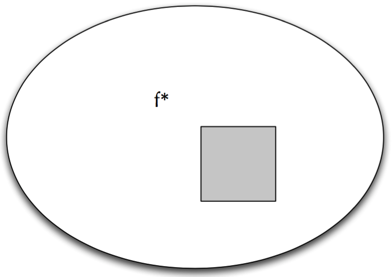
\includegraphics[width=.9\linewidth]{/Users/zhangli/Desktop/论文/UCASthesis/figures/chap01/chap01-pm.png}
\caption{\label{fig:orgparagraph1}
参数模型}
\end{figure}
\end{frame}

\begin{frame}[label={sec:orgheadline8}]{基于HDP的作者主题模型}
\begin{itemize}
\item 是一个非参数模型
\item 不需要进行模型选择,自动产生主题数目\(k\)
\item 当训练数据增加的时候可以进行迭代的训 练,而不需要像主题模型那样重新进行训练以及模型的选择,大大降低了计算资源的消耗
\end{itemize}
\begin{figure}[htb]
\centering
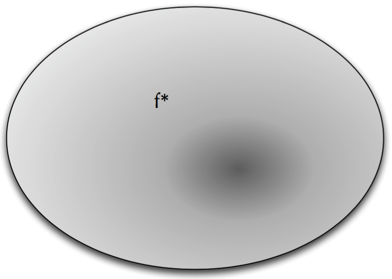
\includegraphics[width=.9\linewidth]{/Users/zhangli/Desktop/论文/UCASthesis/figures/chap01/chap01-npm.png}
\caption{\label{fig:orgparagraph2}
非参数模型}
\end{figure}
\end{frame}

\begin{frame}[label={sec:orgheadline9}]{基于HDP的作者主题模型 (cont.)}
基于HDP的作者主题模型的生成过程如下:

对于每篇文章的每个单词,
\begin{enumerate}
\item 根据均匀分布,在本文档的所有作者中采样一个作者;
\item 根据作者级的Dirichlet process \(G_x\),采样对应主题的词分布\(\phi\)。而\(G_x\)采样自语料级的Dirichlet process \(G_0\);
\item 根据该主题的词分布\(\phi\),生成该词。
\end{enumerate}
\begin{figure}[htb]
\centering
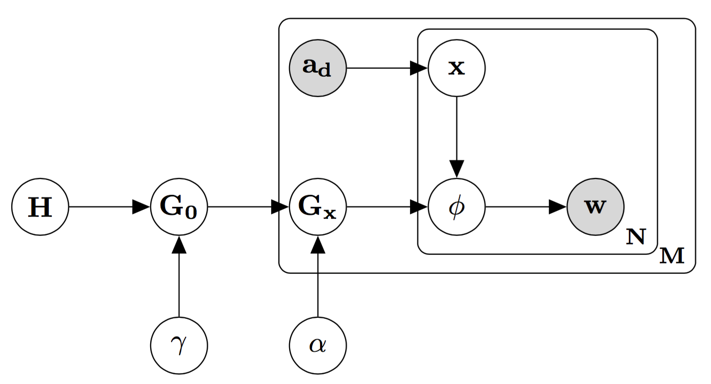
\includegraphics[width=.9\linewidth]{/Users/zhangli/Desktop/论文/UCASthesis/figures/chap01/chap01-natm.png}
\caption{\label{fig:orgparagraph3}
基于HDP的作者主题模型}
\end{figure}
\end{frame}

\begin{frame}[label={sec:orgheadline10}]{评价标准}
混淆度是衡量概率模型训练参数的标准方法。定义如下:
\begin{definition}
\label{def:perplexity}
给定一个单词集合,$(\mathbf{w_d},\mathbf{a_d}),d \in \mathcal{D} ^{test}$,混淆度被定义为:
\begin{equation}
\label{equ:perplexity}
perplexity(\mathbf{w_d},\mathbf{a_d}) = exp[-\frac{lnp(\mathbf{w_d}|\mathbf{a_d})}{N_d}]
\end{equation}
\end{definition}

\begin{align}
\label{equ:prob}
p(\mathbf{w_d}|\mathbf{a_d}) =&\int d\theta \int d\phi p(\theta|\mathcal{D} ^{train})p(\phi | \mathcal{D} ^{train}) \nonumber \\
=& \prod_{m=1}^{N_d}[\frac{1}{A_d}\sum_{i \in \mathbf{a_d},j}\theta_{ij}\phi_{w_mj}]
\end{align}
混淆度越低,模型的泛化越好。
\end{frame}
\begin{frame}[label={sec:orgheadline11}]{实验结果}
\begin{figure}[htb]
\centering
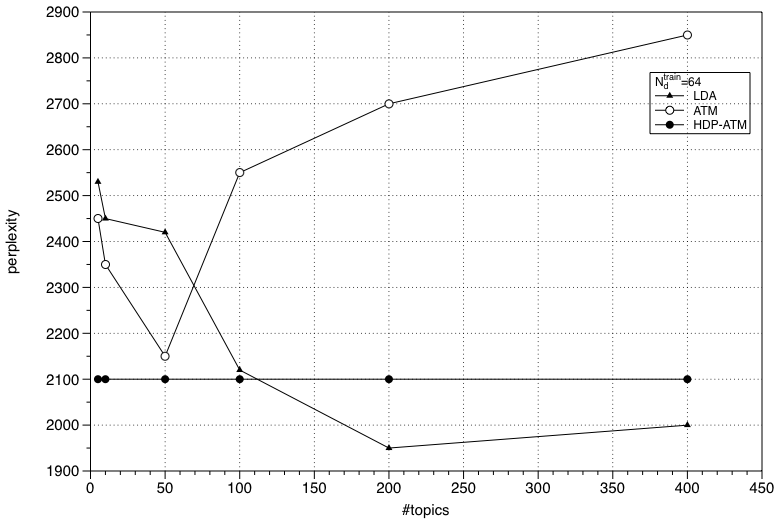
\includegraphics[width=.9\linewidth]{/Users/zhangli/Desktop/论文/UCASthesis/figures/chap01/perplexity64.png}
\caption{\label{fig:orgparagraph4}
模型比较(\(N_d^{train}=64\))}
\end{figure}
\end{frame}

\begin{frame}[label={sec:orgheadline12}]{实验结果}
\begin{figure}[htb]
\centering
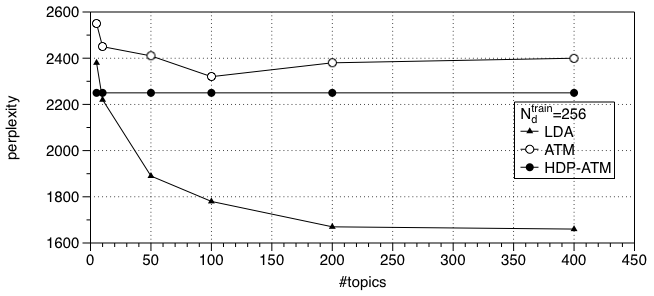
\includegraphics[width=.9\linewidth]{/Users/zhangli/Desktop/论文/UCASthesis/figures/chap01/perplexity256.png}
\caption{\label{fig:orgparagraph5}
模型比较(\(N_d^{train}=256\))}
\end{figure}
\end{frame}

\begin{frame}[label={sec:orgheadline13}]{实验结果}
\begin{figure}[htb]
\centering
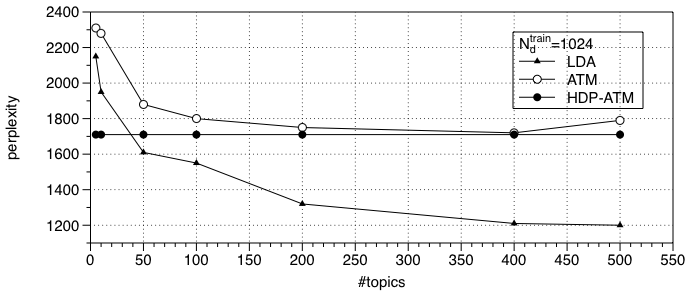
\includegraphics[width=.9\linewidth]{/Users/zhangli/Desktop/论文/UCASthesis/figures/chap01/perplexity1024.png}
\caption{\label{fig:orgparagraph6}
模型比较(\(N_d^{train}=1024\))}
\end{figure}
\end{frame}

\begin{frame}[label={sec:orgheadline14}]{实验结果}
我们可看到,随着主题数的变化(5,10,50,100,200,400,500),
\begin{itemize}
\item 当\(N_d^{train}=64\)时,ATM的在主题数50到100的时候达到最小,而根据实验,当\(N_d^{train}=64\)时,HDP-ATM最后形成的主题数76个,从曲线上符合是ATM的最优值的范围。
\item 同样当\(N_d^{train}=256\)时,ATM的在主题数100到200的时候达到最小,而根据实验,当\(N_d^{train}=256\)时,HDP-ATM最后形成的主题数145个,从曲线上符合是ATM的最优值的范围。
\item 同样当\(N_d^{train}=1024\)时,ATM的在主题数400到500的时候达到最小,而根据实验,当\(N_d^{train}=1024\)时,HDP-ATM最后形成的主题数4个,从曲线上符合是ATM的最优值的范围。
\end{itemize}
\end{frame}
\end{document}
